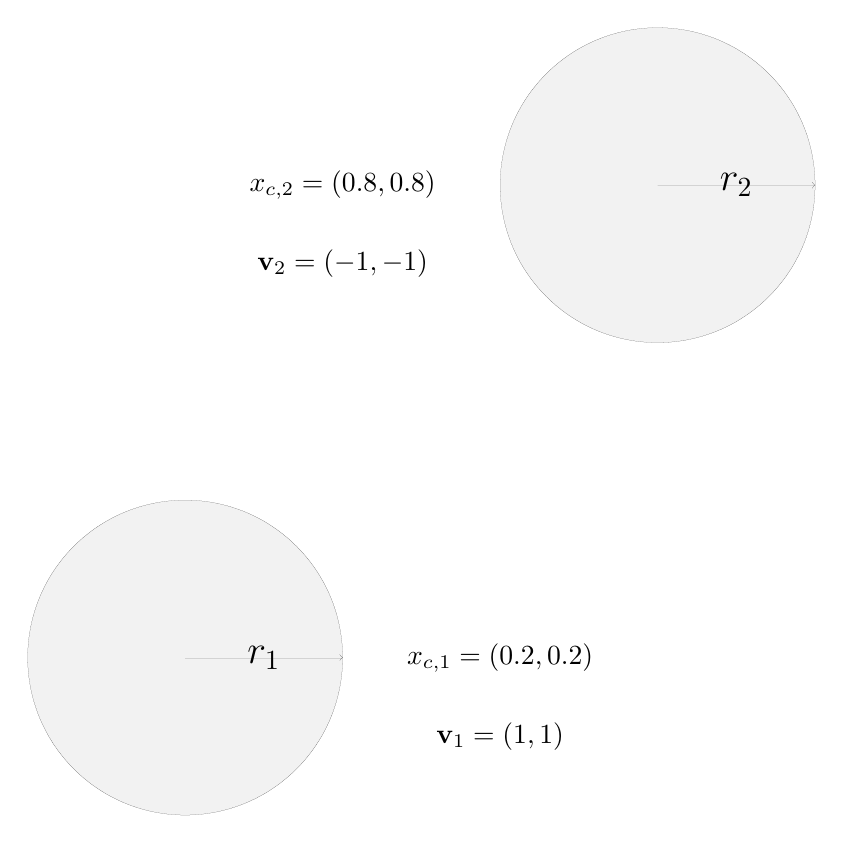
\begin{tikzpicture}[line width=0.001]

  % % draw axes
  % \draw[thick,->,>=stealth] (0,0,0) -- (1,0,0);
  % \draw[thick,->,>=stealth] (0,0,0) -- (0,1,0);
  % \draw[thick,->,>=stealth] (0,0,0) -- (0,0,1);

  % % draw deformed configuration
  % \draw[->,>=stealth] (0,0,0) -- (6.0,3.0,0) node[below, pos=.5] {$\mathbf{x}$};
  % \draw plot [smooth cycle] coordinates {(5,2.25) (6,2.35) (6.5, 2.2) (7,2.5) (7,3.65) (6.5,4.75) (5.8,4.75) (5.3,3.45) (4.8,2.85) };
  % \draw node at (6,3.7) {$\mathcal{B}$};

  % % draw path and displacement
  % % \draw[->,>=stealth] (1.5,3.0,0) -- (6.0,3.0,0) node[above, pos=0.6, font=\small] {$\mathbf{u(X,t)}$};
  % \path[->,>=stealth] (3.1,3.7) edge [bend left] node[above] {$\varphi$} (5.0,3.7);

  % % draw reference configuration
  % % \draw[thick,->,>=stealth] (1.5,3.0,0) -- (2.3,3.4,0) node[pos=1.2] {$\mathbf{N}$};
  % \draw[->,>=stealth] (0,0,0) -- (1.5,3.0,0) node[right, pos=0.6] {$\mathbf{X}$};
  % \draw plot [smooth cycle] coordinates {(1.0,2.1)(1.5,2.2)(2.8,2.5)(2.9,3.5)(2.8,4.8)(1.4,4.5)(0.5,2.5)};
  % \draw node at (1.8,4.2) {$\mathcal{B}_0$};


  \path [draw=black,fill=gray!10] (2,2) circle (2);
  \draw node at (6,2) {\normalsize $x_{c,1} = \left(0.2, 0.2 \right)$};
  \draw node at (6,1) {\normalsize $\mathbf{v}_{1} = \left(1, 1 \right)$};
  \draw[->] (2,2) -- (4,2)  node [midway] {\Large $r_1$};

  \path [draw=black,fill=gray!10] (8,8) circle (2);
  \draw node at (4,8) {\normalsize $x_{c,2} = \left(0.8, 0.8 \right)$};
  \draw node at (4,7) {\normalsize $\mathbf{v}_{2} = \left(-1, -1 \right)$};
  \draw[->] (8,8) -- (10,8)  node [midway] {\Large $r_2$};
  
\end{tikzpicture}
